% Figure 3: Semantic Bottleneck — Task Decomposition vs Functorial Composition
\begin{figure}[t]
\centering
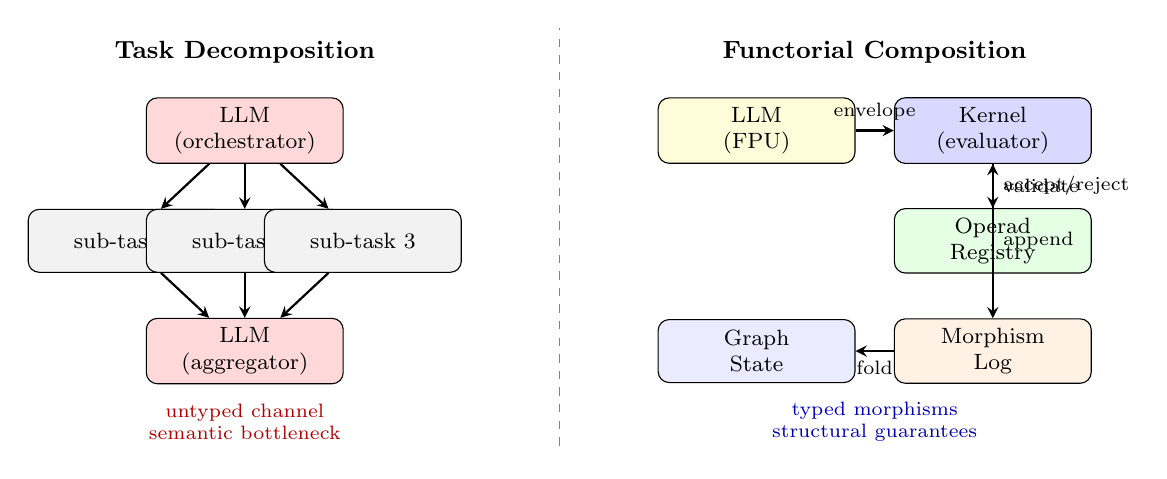
\begin{tikzpicture}[
  box/.style={draw, rounded corners, minimum width=2.5cm, minimum height=0.8cm, align=center, font=\footnotesize},
  arrow/.style={->, thick, >=stealth},
  label/.style={font=\scriptsize}
]

% Left side: Task Decomposition
\node[font=\small\bfseries] at (-4, 4.2) {Task Decomposition};

\node[box, fill=red!15] (llm1) at (-4, 3.2) {LLM\\(orchestrator)};
\node[box, fill=gray!10] (t1) at (-5.5, 1.8) {sub-task 1};
\node[box, fill=gray!10] (t2) at (-4, 1.8) {sub-task 2};
\node[box, fill=gray!10] (t3) at (-2.5, 1.8) {sub-task 3};
\node[box, fill=red!15] (agg) at (-4, 0.4) {LLM\\(aggregator)};

\draw[arrow] (llm1) -- (t1);
\draw[arrow] (llm1) -- (t2);
\draw[arrow] (llm1) -- (t3);
\draw[arrow] (t1) -- (agg);
\draw[arrow] (t2) -- (agg);
\draw[arrow] (t3) -- (agg);

\node[label, text=red!70!black, align=center] at (-4, -0.5) {untyped channel\\semantic bottleneck};

% Divider
\draw[dashed, gray] (0, -0.8) -- (0, 4.5);

% Right side: Functorial Composition
\node[font=\small\bfseries] at (4, 4.2) {Functorial Composition};

\node[box, fill=yellow!15] (fpu) at (2.5, 3.2) {LLM\\(FPU)};
\node[box, fill=blue!15] (kernel) at (5.5, 3.2) {Kernel\\(evaluator)};
\node[box, fill=green!10] (reg) at (5.5, 1.8) {Operad\\Registry};
\node[box, fill=orange!10] (log) at (5.5, 0.4) {Morphism\\Log};
\node[box, fill=blue!8] (state) at (2.5, 0.4) {Graph\\State};

\draw[arrow] (fpu) -- node[above, label] {envelope} (kernel);
\draw[arrow] (kernel) -- node[right, label] {validate} (reg);
\draw[arrow, dashed] (reg) -- node[right, label] {accept/reject} (kernel);
\draw[arrow] (kernel) -- node[right, label] {append} (log);
\draw[arrow] (log) -- node[below, label] {fold} (state);

\node[label, text=blue!70!black, align=center] at (4, -0.5) {typed morphisms\\structural guarantees};

\end{tikzpicture}
\caption{The semantic bottleneck (left): LLMs serve as both orchestrator and
aggregator through an untyped channel, producing brittle compositions.
Functorial composition (right): the LLM acts as a Fuzzy Processing Unit
emitting typed morphism envelopes, validated by the operad registry before
commitment to the append-only log.}
\label{fig:bottleneck}
\end{figure}
